% GGS 662 Assignment 2 -- draft presentation (base your own on this).
% Build (from this folder):
%   pdflatex -interaction=nonstopmode -output-directory=.build assignment2_draft.tex   (run twice)
% Speaker notes: \note{} on each frame. Build assignment2_draft_notes.tex to see them.
% Every number comes from Claude/03_Project/outputs/* and Claude/04_Project/outputs/week4_validation/*.
\documentclass[aspectratio=169,11pt]{beamer}
\usetheme[progressbar=frametitle,numbering=fraction]{metropolis}
\usepackage[T1]{fontenc}
\usepackage{lmodern}
\usepackage{booktabs}
\usepackage{tabularx}
\usepackage{array}
\usepackage{tikz}
\usetikzlibrary{positioning,arrows.meta}
\ifdefined\shownotes
  \usepackage{pgfpages}
  \setbeameroption{show notes on second screen=right}
\fi

\definecolor{navy}{HTML}{14213D}
\definecolor{amber}{HTML}{B45309}
\definecolor{teal}{HTML}{0F766E}
\definecolor{failred}{HTML}{B91C1C}
\definecolor{paper}{HTML}{F7F6F2}
\definecolor{rule}{HTML}{DAD6CC}
\setbeamercolor{frametitle}{bg=navy,fg=paper}
\setbeamercolor{progress bar}{fg=amber,bg=rule}
\setbeamercolor{title separator}{fg=amber}
\setbeamercolor{background canvas}{bg=paper}
\setbeamercolor{block title}{bg=navy!12,fg=navy}
\setbeamercolor{block body}{bg=white}

\newcommand{\todo}[1]{\textcolor{red}{\textbf{TODO: #1}}}
\newcommand{\pass}{\textcolor{teal}{\textbf{PASS}}}
\newcommand{\fail}{\textcolor{failred}{\textbf{FAIL}}}
\newcommand{\nc}{\textcolor{amber}{\textbf{NOT\_CHECKED}}}
\newcommand{\tl}[1]{\texttt{\detokenize{#1}}}
\newcolumntype{Y}{>{\raggedright\arraybackslash}X}
\newcolumntype{R}[1]{>{\raggedleft\arraybackslash}p{#1}}

\title{Verifying an agentic GIS routing workflow}
\subtitle{Fiber route comparison on the shortened Mombasa corridor: baseline, roads, power and rail}
\author{Justin Rogers}
\institute{GGS 662: Agentic GeoAI \quad Assignment 2}
\date{September 28, 2026}

\begin{document}

% ------------------------------------------------------------------ 1
\maketitle
\note{About 15 s. Last week an agent built a fiber-routing workflow for the shortened Mombasa corridor and produced routes, a map and a cost table. This week the question is not whether it ran, but whether the results are correct and defensible. I will give the agent framework briefly, then spend most of the time on the checks and what they found.}

% ------------------------------------------------------------------ 2
\begin{frame}{Agent framework: six dimensions (04\_01)}
\footnotesize
\begin{columns}[T,onlytextwidth]
\column{0.32\textwidth}
\begin{block}{Goal}Compare baseline, roads, power and rail routes between the exact \tl{route1_short} endpoints (east = start); report length and USD 10/m cost.\end{block}
\begin{block}{Agency}Agent cleans, nodes, repairs gaps and routes. \textbf{Human} fixed endpoints, 50\,m gap limit, 500\,m endpoint limit and the rate.\end{block}
\column{0.32\textwidth}
\begin{block}{Environment}Saved 03\_01 GeoPackages, AGENTS.md rules, 3{,}000\,m study rectangle, measured in EPSG:32737. No new downloads.\end{block}
\begin{block}{Feedback}Stop with \tl{endpoint_too_far}, \tl{no_path} or \tl{empty_network}. A failed check means revise, never relax a threshold.\end{block}
\column{0.32\textwidth}
\begin{block}{Tools}geopandas, shapely, networkx (Dijkstra), pandas; matplotlib + contextily for maps.\end{block}
\begin{block}{Verification}Independent audit script, synthetic cases, controlled reruns. Real-world claims need imagery or authoritative data.\end{block}
\end{columns}
\note{About 40 s. Goal: four candidate routes between the exact endpoints of the shortened baseline, easterly point as start, with length and a classroom cost of 10 dollars per metre. Environment: only the saved 03\_01 files and the AGENTS.md rules. Tools: geopandas, shapely, networkx. Agency: the agent chooses how to clean, node, repair and route, but a human set the endpoints, the 50 m gap limit, the 500 m endpoint limit and the rate. Feedback: stop with a named status rather than invent a route; a failed check means revise, not raise a threshold. Verification: an audit that recomputes everything from saved files, plus outside evidence for real-world claims.}
\end{frame}

% ------------------------------------------------------------------ 3
\begin{frame}{Where the human decides and where the agent revises}
\small
\begin{columns}[T,onlytextwidth]
\column{0.48\textwidth}
\begin{block}{Stays with a human}
Whether an inferred connector or a 2D crossing is actually buildable, and which corridor to pursue.\\[4pt]
Access rights, permits and engineering feasibility are not in the data, so the agent cannot establish them.
\end{block}
\column{0.48\textwidth}
\begin{block}{Feedback that changes the next action}
The audit flags the rail route switching lines at a bridge ($-3.99374$, $39.54626$) with no shared OSM node.\\[4pt]
If imagery shows the lines are grade-separated: \textbf{remove that transfer and reroute rail}, then report the new length or \tl{no_path}. Do not raise a threshold to keep the old answer.
\end{block}
\end{columns}
\note{About 25 s. One decision that must stay human: whether anything the model inferred, a connector or a crossing, can actually be built, and which corridor to pursue; that depends on access rights and engineering that are not in the data. One piece of feedback that should change the agent's next action: the audit found the rail route switching onto a bridge where the two lines share no OSM node. If imagery confirms they are at different levels, the agent should delete that transfer and reroute, accepting a longer route or no\_path, rather than loosening a threshold.}
\end{frame}

% ------------------------------------------------------------------ 4
\begin{frame}{Approach: checks designed around the agent, not after it}
\centering
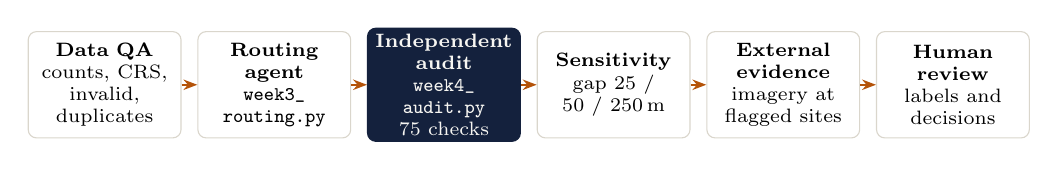
\begin{tikzpicture}[
  box/.style={draw=rule, fill=white, rounded corners=3pt, align=center, text width=1.8cm, minimum height=1.35cm, inner sep=2pt, font=\scriptsize},
  hi/.style={box, fill=navy, draw=navy, text=paper},
  arr/.style={-{Stealth[length=5pt]}, thick, amber}]
\node[box] (a) {\textbf{Data QA}\\counts, CRS, invalid, duplicates};
\node[box, right=0.2cm of a] (b) {\textbf{Routing agent}\\\tl{week3_}\\\tl{routing.py}};
\node[hi, right=0.2cm of b] (c) {\textbf{Independent}\\\textbf{audit}\\\tl{week4_}\\\tl{audit.py}\\75 checks};
\node[box, right=0.2cm of c] (d) {\textbf{Sensitivity}\\gap 25 / 50 / 250\,m};
\node[box, right=0.2cm of d] (e) {\textbf{External evidence}\\imagery at flagged sites};
\node[box, right=0.2cm of e] (f) {\textbf{Human review}\\labels and decisions};
\foreach \x/\y in {a/b,b/c,c/d,d/e,e/f} \draw[arr] (\x) -- (\y);
\end{tikzpicture}

\vspace{10pt}
\small
\begin{columns}[T,onlytextwidth]
\column{0.48\textwidth}
\textcolor{teal}{\textbf{Independent of the code.}} The audit never imports the routing script; it recomputes every value from the saved files and the 03\_01 inputs.
\column{0.48\textwidth}
\textcolor{amber}{\textbf{Not independent of the author.}} The same AI tool wrote both scripts, so the audit verifies computations. Real-world claims need outside evidence.
\end{columns}
\note{About 25 s. I followed the 04\_02 validation stack: data QA, the routing agent, then a separate audit script that imports no routing code and rebuilds every length, cost and connector from the saved files; controlled reruns that change only the gap tolerance; outside evidence at the sites the audit flags; and a human applies the labels. Caveat: the same AI tool wrote both scripts, so the audit is verification, not independent validation.}
\end{frame}

% ------------------------------------------------------------------ 5
\begin{frame}{Route map: what the agent built and what it inferred}
\begin{columns}[T,onlytextwidth]
\column{0.56\textwidth}
\centering
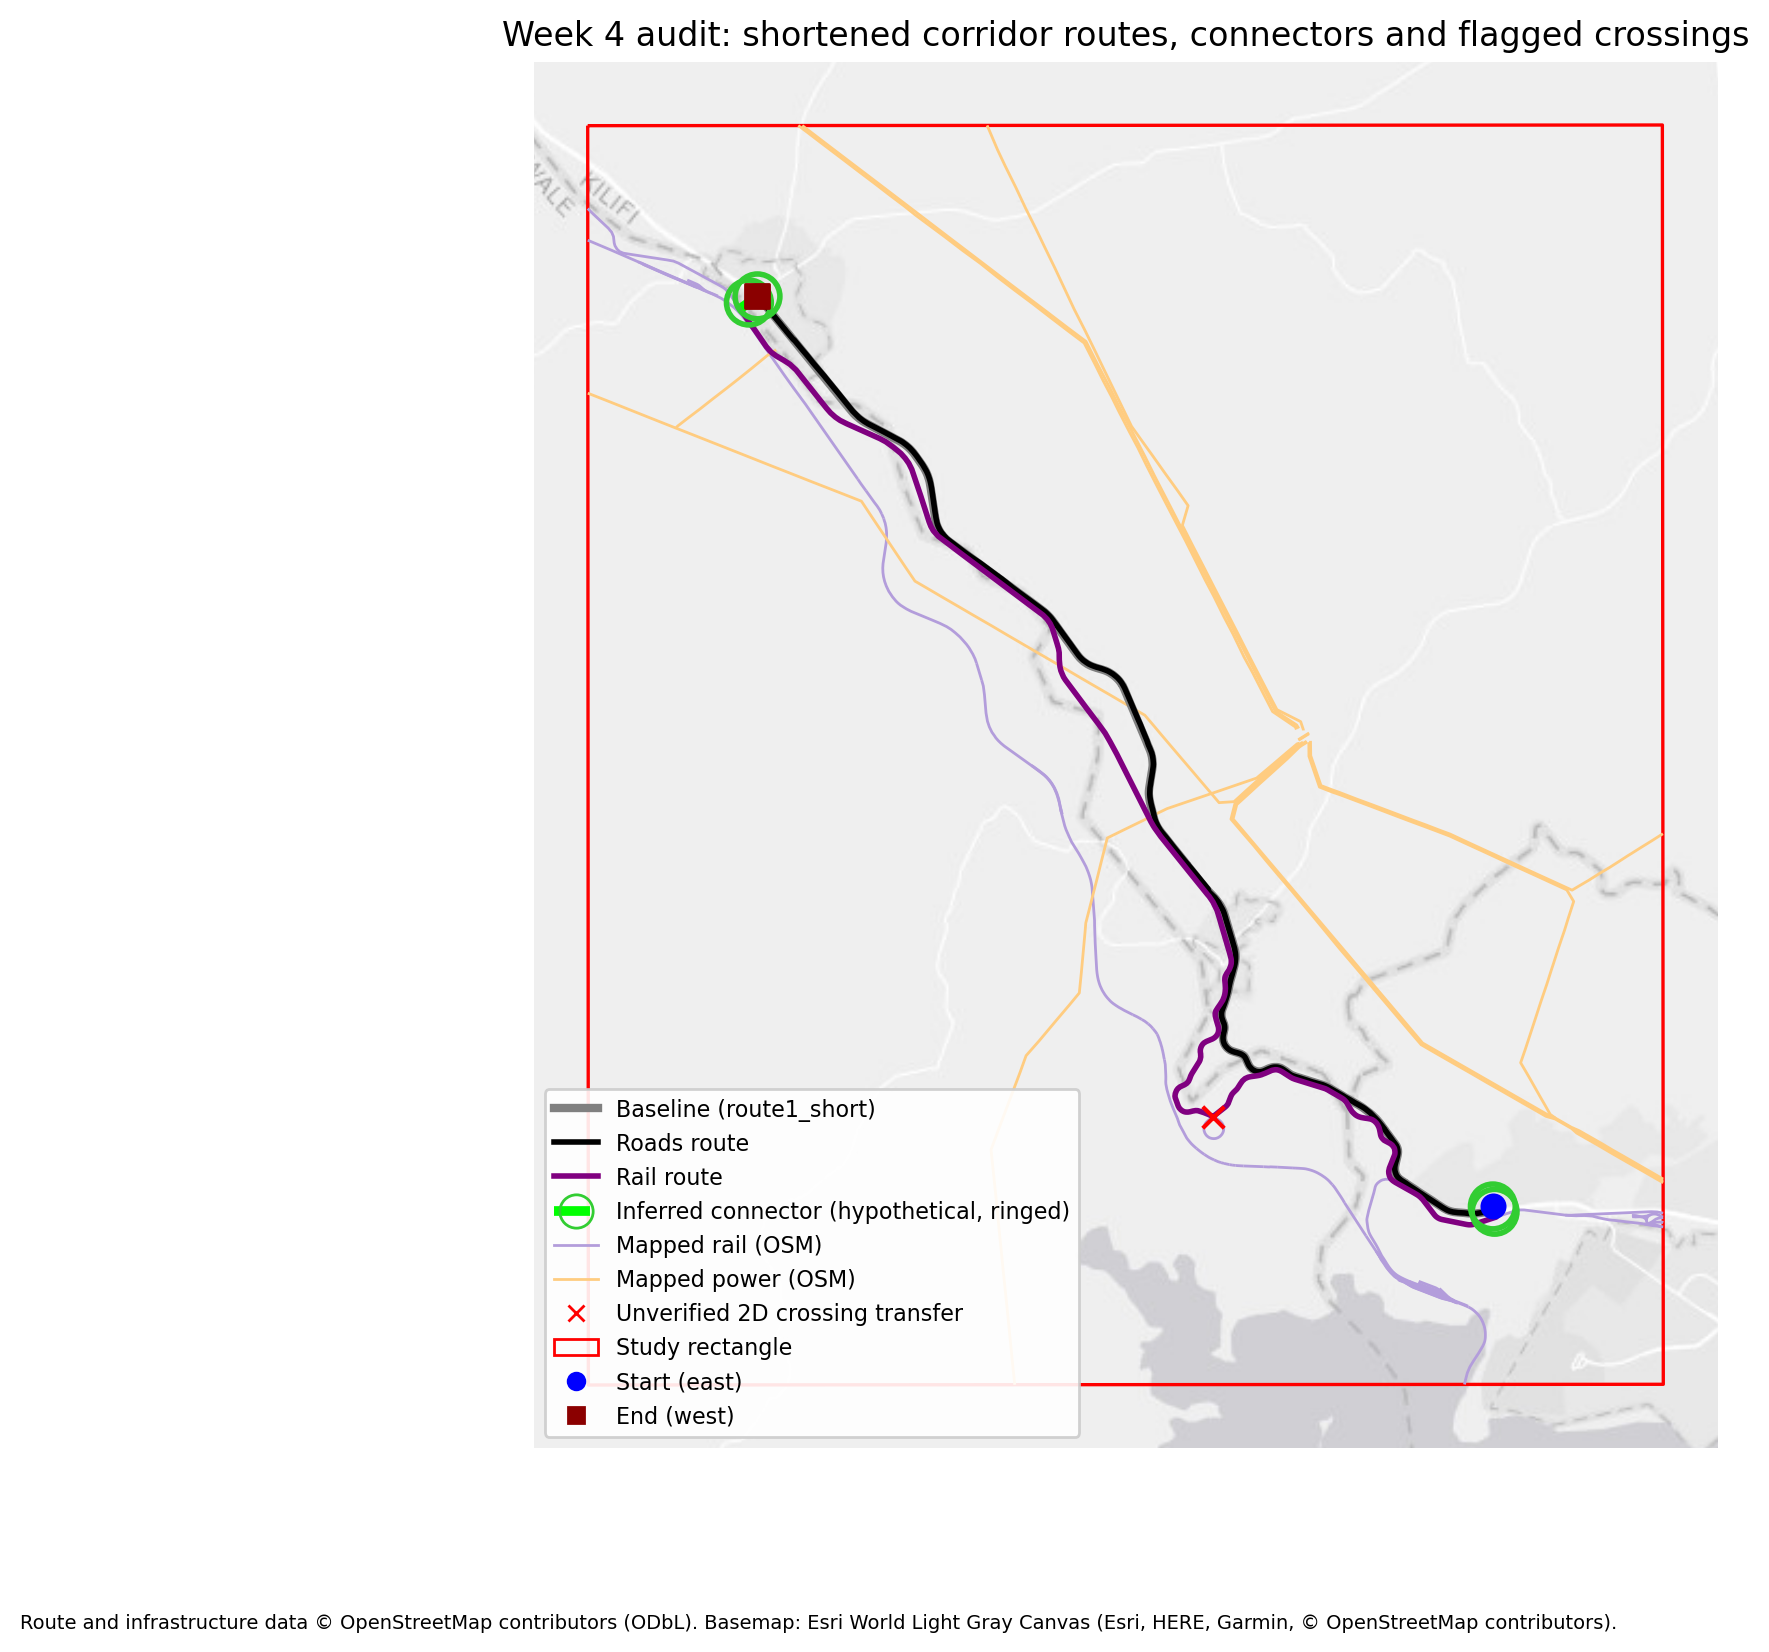
\includegraphics[height=0.76\textheight,keepaspectratio]{../outputs/week4_validation/validation_map.png}
\column{0.42\textwidth}
\footnotesize
\textcolor{teal}{\textbf{Green rings: inferred connectors.}} Roads 0.59\,m and 0.72\,m; rail 194.8\,m and 372.7\,m. All four are endpoint connectors: hypothetical new construction.

\vspace{6pt}
\textcolor{failred}{\textbf{Red cross: flagged crossing.}} The rail route switches onto a bridge-tagged line where the two lines share no OSM vertex.

\vspace{6pt}
\textcolor{navy}{\textbf{Lengths.}} Baseline 22{,}896.8\,m; roads 22{,}897.6\,m; rail 25{,}902.4\,m. Power: \tl{endpoint_too_far}.

\vspace{6pt}
\scriptsize Data \copyright\ OpenStreetMap contributors (ODbL). Basemap: Esri World Light Gray Canvas.
\end{columns}
\note{About 35 s. Grey baseline and black roads route overlap almost everywhere, under one metre apart in total length. Purple is rail, 3 km longer. Green rings mark every place the model invented geometry: two sub-metre snaps for roads, and 195 m and 373 m links for rail, all endpoint connectors, drawn separately from mapped infrastructure. The red cross is where the rail route jumps onto a bridge at a point with no shared node, the one failed check. Power has no route: its start is 1.8 km from any mapped power line.}
\end{frame}

% ------------------------------------------------------------------ 6
\begin{frame}{Verification evidence: 75 reproducible checks}
\small
\begin{columns}[T,onlytextwidth]
\column{0.32\textwidth}\centering{\LARGE\textcolor{teal}{\textbf{71}}}\\PASS
\column{0.32\textwidth}\centering{\LARGE\textcolor{failred}{\textbf{1}}}\\FAIL: 2D crossing at a bridge
\column{0.32\textwidth}\centering{\LARGE\textcolor{amber}{\textbf{3}}}\\NOT\_CHECKED: external evidence
\end{columns}
\vspace{2pt}
\scriptsize
\begin{tabularx}{\textwidth}{@{}l R{0.9cm} R{0.9cm} R{1.5cm} Y@{}}
\toprule
Category & PASS & FAIL & NOT\_CHK & What it checks\\
\midrule
Provenance and data QA & 7 & 0 & 0 & counts, CRS, invalid geometry, duplicates\\
Comparison table and cost & 9 & 0 & 0 & four rows, blank unavailable values, length $\times$ USD 10/m\\
Route geometry and length & 23 & 0 & 0 & endpoints, continuity, metres, edge sum within 0.01\,m\\
Connectors & 6 & 0 & 0 & limits, containment, counted once\\
Unavailable route (power) & 1 & 0 & 0 & endpoint distance recomputed\\
Synthetic cases & 20 & 0 & 0 & 6 cases $\times$ 3 runs, plus the 230\,m oracle\\
Sensitivity & 5 & 0 & 0 & only the gap setting changed\\
Spatial assumption & 0 & \textcolor{failred}{1} & 0 & route transfers only at OSM junctions\\
External evidence & 0 & 0 & \textcolor{amber}{3} & imagery at flagged sites (pending)\\
\bottomrule
\end{tabularx}
\note{About 35 s. Each check records method, expected, observed, evidence file and PASS, FAIL or NOT\_CHECKED; missing evidence never counts as a pass. The computational checks all pass: exact endpoints, geometry length equal to the traversed-edge sum within 1 cm, metres not degrees (UTM within 0.036\% of geodesic), cost equals length times 10, connectors counted once. Synthetic cases cover the five AGENTS.md situations plus connector-counted-once in all three runs, and a hand oracle: 80 + 120 + 30 m gap = 230 m and USD 2,300. One fail and three not-checked are the interesting ones.}
\end{frame}

% ------------------------------------------------------------------ 7
\begin{frame}{What the checks caught}
\small
\begin{columns}[T,onlytextwidth]
\column{0.48\textwidth}
\begin{block}{\textcolor{failred}{FAIL}: a 2D crossing at a rail bridge}
The route moves from way 891041250 onto bridge-tagged way 239559205 at ($-3.993745$, $39.54626$); neither line has a vertex there. A modelling assumption, not a proven error: needs imagery.
\end{block}
\begin{block}{A bug in the agent's own checker}
The connector-limit check hard-coded 50\,m, so the 250\,m rerun was checked against the wrong limit. It now reads the run's setting.
\end{block}
\column{0.48\textwidth}
\begin{block}{A wrong claim in the Week 3 answers}
The write-up said rail used a gap connector. \tl{connectors.gpkg} shows all four used connectors are endpoint connectors (rail: 194.8\,m and 372.7\,m). Corrected.
\end{block}
\begin{block}{\textcolor{teal}{A justified failure}: power}
\tl{endpoint_too_far} confirmed independently: start 1{,}839.2\,m and end 995.1\,m from the nearest mapped power line, against a 500\,m limit.
\end{block}
\end{columns}
\note{About 45 s. First, the one failure: the audit looks for places where the route changes from one OSM line to another at a point that is not a shared vertex, which is exactly where "2D crossings connect" can be wrong. It found one, on a bridge-tagged rail line. Second, the agent's own Week 3 discussion claimed rail used a gap connector; the saved connectors file shows all four are endpoint connectors, so the prose was wrong though the numbers were right. Third, the built-in check hard-coded 50 m and would have mis-checked the 250 m rerun. Fourth, a justified no-route result: power really is 1.8 km from the start. A successful run alone would have hidden the first three.}
\end{frame}

% ------------------------------------------------------------------ 8
\begin{frame}{Sensitivity: changing only the gap tolerance changes no route outcome}
\scriptsize
\begin{tabularx}{\textwidth}{@{}l l l l R{1.6cm} Y@{}}
\toprule
Gap tolerance & Roads & Power & Rail & Power parts$^{*}$ & Ranking\\
\midrule
25\,m & ok, 22{,}897.6\,m & \tl{endpoint_too_far} & ok, 25{,}902.4\,m & 6 & baseline $<$ roads $<$ rail\\
50\,m (original) & ok, 22{,}897.6\,m & \tl{endpoint_too_far} & ok, 25{,}902.4\,m & 3 & baseline $<$ roads $<$ rail\\
250\,m & ok, 22{,}897.6\,m & \tl{endpoint_too_far} & ok, 25{,}902.4\,m & 1 & baseline $<$ roads $<$ rail\\
\bottomrule
\end{tabularx}

\scriptsize $^{*}$Power connected components after gap repair (9 before). Runs: \tl{sensitivity_gap_25m}, \tl{default}, \tl{gap_tolerance_250m}.

\vspace{6pt}\footnotesize
\begin{columns}[T,onlytextwidth]
\column{0.48\textwidth}
\textbf{Why nothing moves.} No route uses a gap connector, and power fails on the 1{,}839\,m endpoint distance, which no gap setting can fix. Connector counts and lengths are identical in all three runs.
\column{0.48\textwidth}
\textbf{What this does not show.} One setting at three values is not global robustness (Saltelli et al., 2019). A common rate of USD 5, 10 or 20/m scales costs but keeps the same order.
\end{columns}
\note{About 30 s. The rerun changes only the gap tolerance, and the audit confirms nothing else in the settings changed. At 25, 50 and 250 m every status, length, connector and the ranking are identical. Only the power layer's internal fragmentation responds: 9 raw pieces become 6, 3 or 1. So the power failure is not a threshold artefact. Limit: a single-parameter rerun cannot show robustness to the endpoint limit or the crossing rule.}
\end{frame}

% ------------------------------------------------------------------ 9
\begin{frame}{Conclusions: what I trust and what stays unresolved}
\scriptsize
\begin{tabularx}{\textwidth}{@{}Y >{\raggedright\arraybackslash}p{5.4cm} l@{}}
\toprule
Conclusion & Label (04\_02 \S16) & Evidence\\
\midrule
Lengths, endpoints, containment and costs are computed correctly & \textcolor{teal}{\textbf{VERIFIED}} & R-*, C-*\\
Connectors within limits, counted once; all are endpoint connectors & \textcolor{teal}{\textbf{VERIFIED}} & R-*-conn*\\
Power unavailable because its start is 1{,}839\,m from mapped lines & \textcolor{teal}{\textbf{VERIFIED}}; a real line there: \textbf{UNRESOLVED} & U-power\\
Ranking baseline $<$ roads $<$ rail holds for a 25--250\,m gap tolerance & not \textbf{SENSITIVE} to this one setting & S-*\\
The rail transfer at the bridge is buildable & \textcolor{failred}{\textbf{UNRESOLVED}} (check failed) & V-crossings\\
Connector sites and the crossing match conditions on the ground & \todo{PENDING imagery} & E-*\\
Access rights, permits, feasibility and real costs & \textcolor{failred}{\textbf{UNRESOLVED}} & none in data\\
\bottomrule
\end{tabularx}

\vspace{4pt}
\footnotesize\todo{Add your imagery screenshots of the 3 sites in \tl{external_evidence.csv}, rerun \tl{week4_audit.py}, then relabel the E-* row EXTERNALLY SUPPORTED or UNRESOLVED.}
\note{About 35 s. What I trust: the computations are verified, and the power failure is real under this data. The ranking does not depend on the gap tolerance. What I do not trust yet: the rail transfer at the bridge, which failed the crossing check, and whether the connector sites look the way the model assumes. \todo{say what your imagery showed.} Nothing here establishes access rights, permits or real costs; proximity is not permission, and 10 dollars per metre is a classroom value. Verified, not yet validated.}
\end{frame}

% ------------------------------------------------------------------ 10
\begin{frame}[shrink=12]{Sources and AI use}
\scriptsize
\begin{columns}[T,onlytextwidth]
\column{0.5\textwidth}
\textbf{\small Data, tools and readings}
\begin{itemize}
\item Roads, rail, power, settlements: \copyright\ OpenStreetMap contributors, ODbL (saved in 03\_01).
\item Basemaps: Esri World Light Gray Canvas and World Street Map (Esri, HERE, Garmin, \copyright\ OpenStreetMap contributors).
\item GGS 662 notebooks 03\_01, 03\_02, 04\_01, 04\_02 and AGENTS.md. Python: geopandas, shapely, networkx, pandas, pyproj.
\item Oreskes, Shrader-Frechette \& Belitz (1994), \emph{Science}, doi:10.1126/science.263.5147.641
\item Haklay (2010), \emph{Environment and Planning B}, doi:10.1068/b35097
\item Saltelli et al. (2019), \emph{Environmental Modelling \& Software}, doi:10.1016/j.envsoft.2019.01.012
\end{itemize}
\column{0.46\textwidth}
\begin{block}{AI-use statement \quad \todo{EDIT IN YOUR OWN WORDS}}
I used Claude Code (Anthropic, Claude Opus 5.5) to write the Week 3 routing script and the Week 4 audit script, to review both for errors, and to draft these slides. The audit caught a hard-coded connector limit and a wrong claim in the tool's own Week 3 write-up.\\[4pt]
I reviewed and ran every script, checked the flagged sites in imagery, and edited the slides. Because the same tool wrote the code and the audit, I treat the audit as verification, not independent validation.
\end{block}
\end{columns}
\note{About 10 s. Data from OpenStreetMap contributors under ODbL, with Esri basemaps. Readings are the three from 04\_02 that shaped the audit. \todo{rewrite the AI statement in your own words and make sure every claim in it is true, including the imagery check.}}
\end{frame}

% ================================================================== supporting
\appendix
\begin{frame}[standout]
Supporting slides\\[4pt]
{\normalsize Full check table, synthetic cases and evidence files}
\end{frame}

\begin{frame}{Supporting: per-route checks (all PASS)}
\scriptsize
\begin{tabularx}{\textwidth}{@{}Y l l l@{}}
\toprule
Check (tolerance) & Baseline & Roads & Rail\\
\midrule
Valid, nonempty single LineString & PASS & PASS & PASS\\
Endpoints match baseline ($\le$0.01\,m) & 0.0000 / 0.0000\,m & 0.0000 / 0.0000\,m & 0.0000 / 0.0000\,m\\
No loops or self-crossing (\tl{is_simple}) & True & True & True\\
Inside study rectangle & True & True & True\\
Geometry vs traversed-edge sum ($\le$0.01\,m) & 0.000000\,m & 0.009833\,m & 0.007000\,m\\
Metres not degrees (UTM vs geodesic, $<$0.1\%) & $-0.036$\% & $-0.036$\% & $-0.036$\%\\
Not shorter than straight line & 1.111$\times$ & 1.111$\times$ & 1.257$\times$\\
Cost = length $\times$ USD 10/m & 228{,}967.56 & 228{,}975.93 & 259{,}023.67\\
Connectors counted once (count, total) & 0, 0\,m & 2, 1.3139\,m & 2, 567.5396\,m\\
Each connector $\le$500\,m, inside, on route, at endpoint & -- & 0.59, 0.72\,m & 194.85, 372.69\,m\\
Non-connector length on mapped lines ($\pm$1\,m) & -- & 22{,}896.4\,m & 25{,}334.9\,m\\
\bottomrule
\end{tabularx}

\vspace{4pt}\tiny Source: \tl{validation_table.csv} (R-* checks). Note: roads edge-sum difference (0.0098\,m) passes but sits close to the 0.01\,m tolerance, consistent with 1\,cm node rounding.
\end{frame}

\begin{frame}{Supporting: provenance, data QA and comparison table}
\scriptsize
\begin{tabularx}{\textwidth}{@{}l Y l@{}}
\toprule
Check ID & Observed & Status\\
\midrule
P-settings & Settings match spec: gap 50\,m, endpoint 500\,m, margin 3{,}000\,m, EPSG:32737 & \pass\\
D-roads & 4{,}742 features, EPSG:4326, 0 missing / empty / invalid, all intersect study area & \pass\\
D-power & 15 features, 0 missing / empty / invalid & \pass\\
D-rail & 77 features, 0 missing / empty / invalid & \pass\\
D-baseline & 1 LineString, valid & \pass\\
D-settlements & 30 features (29 points, 1 polygon), map context only & \pass\\
D-roads-dup & 2{,}292 of 4{,}742 edges are reversed OSMnx duplicates; removed before routing & \pass\\
C-rows & baseline, roads, power, rail: one row each & \pass\\
C-cols & nine required CSV columns & \pass\\
C-base & baseline connector values 0, 0, 0 & \pass\\
C-unavail & power: \tl{endpoint_too_far}, blank length and cost (not zero) & \pass\\
C-gpkg & \tl{routes.gpkg} holds baseline, roads, rail & \pass\\
\bottomrule
\end{tabularx}
\end{frame}

\begin{frame}{Supporting: unavailable route, spatial assumption, sensitivity, external evidence}
\scriptsize
\begin{tabularx}{\textwidth}{@{}l Y l@{}}
\toprule
Check ID & Observed & Status\\
\midrule
C-rate & one common rate, USD 10/m & \pass\\
U-power & start 1{,}839.2\,m, end 995.1\,m from nearest power line ($>$500\,m) & \pass\\
V-crossings & 1 transfer at a non-shared vertex; involves a bridge-tagged way & \fail\\
S-25m-ctrl & only ``Gap connector limit'' changed, 50 $\to$ 25\,m & \pass\\
S-25m-out & no differences; ranking unchanged; power parts 6 & \pass\\
S-250m-ctrl & only ``Gap connector limit'' changed, 50 $\to$ 250\,m & \pass\\
S-250m-out & no differences; ranking unchanged; power parts 1 & \pass\\
S-rate & same order at USD 5, 10, 20/m & \pass\\
E-rail connector 3 & 195\,m connector site ($-4.008849$, $39.591099$): no evidence yet & \nc\\
E-rail connector 4 & 373\,m connector site ($-3.864413$, $39.472359$): no evidence yet & \nc\\
E-rail crossing 1 & crossing site ($-3.993745$, $39.54626$): no evidence yet & \nc\\
\bottomrule
\end{tabularx}

\vspace{4pt}\small\todo{Fill in \tl{external_evidence.csv} (source, date, provenance, independent\_of\_osm, observation, supports\_claim) and rerun the audit.}
\end{frame}

\begin{frame}{Supporting: synthetic cases and known-answer oracle}
\scriptsize
\begin{tabularx}{\textwidth}{@{}Y l l l l@{}}
\toprule
Case (AGENTS.md) & Expected & 50\,m run & 25\,m run & 250\,m run\\
\midrule
Already connected: components & 1 & 1 \pass & 1 \pass & 1 \pass\\
Gap below threshold: components after repair & 1 & 1 \pass & 1 \pass & 1 \pass\\
Gap above threshold: components after repair & 2 & 2 \pass & 2 \pass & 2 \pass\\
Endpoint on a line interior: status & ok & ok \pass & ok \pass & ok \pass\\
Disconnected endpoints: status & \tl{no_path} & \tl{no_path} \pass & \tl{no_path} \pass & \tl{no_path} \pass\\
Connector counted once: route length (10\,m + gap + 20\,m) & = expected & 55.0\,m \pass & 42.5\,m \pass & 155.0\,m \pass\\
\midrule
Oracle: 80\,m + 120\,m + 30\,m gap at USD 10/m & 230\,m, USD 2{,}300 & \multicolumn{3}{l}{230\,m, USD 2{,}300 \pass}\\
Oracle fault: gap double-counted & flagged & \multicolumn{3}{l}{260\,m $\neq$ 230\,m flagged \pass}\\
\bottomrule
\end{tabularx}

\vspace{4pt}\tiny The gap in the connector case is half the run's tolerance, so the expected length differs per run. Source: \tl{routing_report.md} in each run folder; audit IDs T-*.
\end{frame}

\begin{frame}[fragile]{Supporting: evidence files, run commands and versions}
\scriptsize
\textbf{Run commands} (every argument has a default)
\begin{itemize}
\item \tl{python Claude/03_Project/week3_routing.py} $\to$ \tl{outputs/default/}
\item \verb|python week3_routing.py --gap-tolerance-m 25 --out outputs/sensitivity_gap_25m|
\item \verb|python week3_routing.py --gap-tolerance-m 250 --out outputs/gap_tolerance_250m|
\item \tl{python Claude/04_Project/week4_audit.py} $\to$ \tl{outputs/week4_validation/}
\end{itemize}
\textbf{Evidence files}
\begin{itemize}
\item Each run folder: \tl{route_comparison.csv}, \tl{routes.gpkg}, \tl{connectors.gpkg}, \tl{route_map.png}, \tl{routing_report.md}
\item \tl{Claude/04_Project/outputs/week4_validation/}: \tl{validation_table.csv}, \tl{validation_report.md}, \tl{validation_map.png}, \tl{inferred_crossings.gpkg}, \tl{external_evidence.csv}
\end{itemize}
\textbf{Versions}: Python 3.12.2; geopandas 1.1.4; shapely 2.1.2; pyproj 3.8.0; networkx 3.6.1; pandas 2.3.3.\\[4pt]
\textbf{Output location}: 04\_02 names \tl{outputs/week3_routing/} and \tl{outputs/week4_validation/} at the repo root; these are kept under \tl{Claude/} so the course repo inputs stay read-only.
\end{frame}

\end{document}
